\documentclass[pdftex,11pt,a4paper]{article}
\usepackage{blindtext}
\usepackage{graphicx}
\usepackage{subfiles}
\usepackage{amsmath}
\usepackage{amsthm}
\usepackage{tikz}
\usepackage{wrapfig}
\usepackage{lscape}
\usepackage{rotating}
\usepackage{epstopdf}
\usepackage[font=small,labelfont=bf]{caption}
\usepackage{hyperref}
\hypersetup{
    colorlinks=true,
    linkcolor=blue,
    citecolor=blue
}
\usetikzlibrary{shapes.geometric, arrows}
\theoremstyle{definition}
\newtheorem{definition}{Definition}[section]
\newtheorem{theorem}{Theorem}[section]
\newtheorem{lemma}[theorem]{Lemma}
\theoremstyle{remark}
\newtheorem*{remark}{Remark}
\usepackage{amssymb}
\usepackage{amsfonts}
\usepackage{mathtools}
\usepackage{geometry}
 \geometry{
 a4paper,
 total={210mm,297mm},
 left=30mm,
 right=30mm,
 top=30mm,
 bottom=35mm,
 }
\newcommand{\defeq}{\vcentcolon=}
\newcommand{\eqdef}{=\vcentcolon}
\newcommand*{\V}[1]{\mathbf{#1}}%
\newcommand{\norm}[1]{\left\lVert#1\right\rVert}
\newcommand{\justif}[2]{&{#1}&\text{#2}}
\newcommand{\qedwhite}{\hfill \ensuremath{\Box}}
\newcommand\given[1][]{\:#1\vert\:}
\newcommand{\me}{\mathrm{e}}
\DeclarePairedDelimiterX{\infdivx}[2]{(}{)}{%
  #1\;\delimsize\|\;#2%
}
\newcommand{\Conv}{\mathop{\scalebox{1.5}{\raisebox{-0.2ex}{$\ast$}}}}%
\newcommand{\infdiv}{\infdivx}
\renewcommand{\qed}{\hfill\blacksquare}
\hyphenation{op-tical net-works semi-conduc-tor tech-no-lo-gy}


\begin{document}
\title{Learning relational structures from birdsong}
\author{Authors,~a}

\maketitle


\begin{abstract}
We infer phylo-acoustic trees (relational structures built from acoustic similarity) for over 80 bird species in the British Isles. We characterise each bird species as a Variational Bayes Hidden Markov Model trained on birdsong excerpts and then use their pairwise similarity to build a phylo-acoustic tree by running Agglomerative Hierarchical Clustering. In order to achieve this, we define similarity metrics for HMMs, hence implicitly defining a \emph{length-invariant} method to compare birdsong across different species. Additionally, we show that there is a clear community structure in the resulting phylo-acoustic trees.
\end{abstract}


\section{Introduction (500 words)}
The explosion of data in recent years has allowed scientists to gain insight in a diversity of domains. Furthermore, the widespread use of computational methods has in turn provided means of rapidly extracting conclusions from data. For example, environmental scientists have been allowed to contribute to quantify environments by means of \emph{unsupervised learning} techniques, which aim to provide insight on the hidden structures of data. Quantifying environments is crucial in order to analyse phenomena in a formal manner.
\par In this work, we tackle the problem of describing a hierarchical structure of bird species only by means of their birdsong. This mathematical representation relies only on the validity of a formal analysis framework, and hence unveils relations that go beyond empirical conclusions. This phylo-acoustic tree may further our understanding of relations among bird species in a large geographical area, and bird evolution over a large span of time. 
\par Moreover, birdsong is a rich means of communication that encapsulates behavioural patterns (such as territory defence and mate attraction or competition \cite{Berwick2013, Naguib2014}) in a regular and hierarchical fashion, as shown in figure \ref{fig_birdsong_structure}. Crucially, birdsong is learnt by repetition \cite{Berwick2013}, which implies that forced migration may push flocks to learn songs that do not necessarily come from their parents. However, given a species whose birdsong has not suffered too much from this phenomenon, it might be possible to trace back the evolutionary links of bird species. On the other hand, the loss of natural habitats (which increases forced migration) may also leave us forever with questions unanswered \cite{Marler2004}.
\begin{figure}[t]
\centering
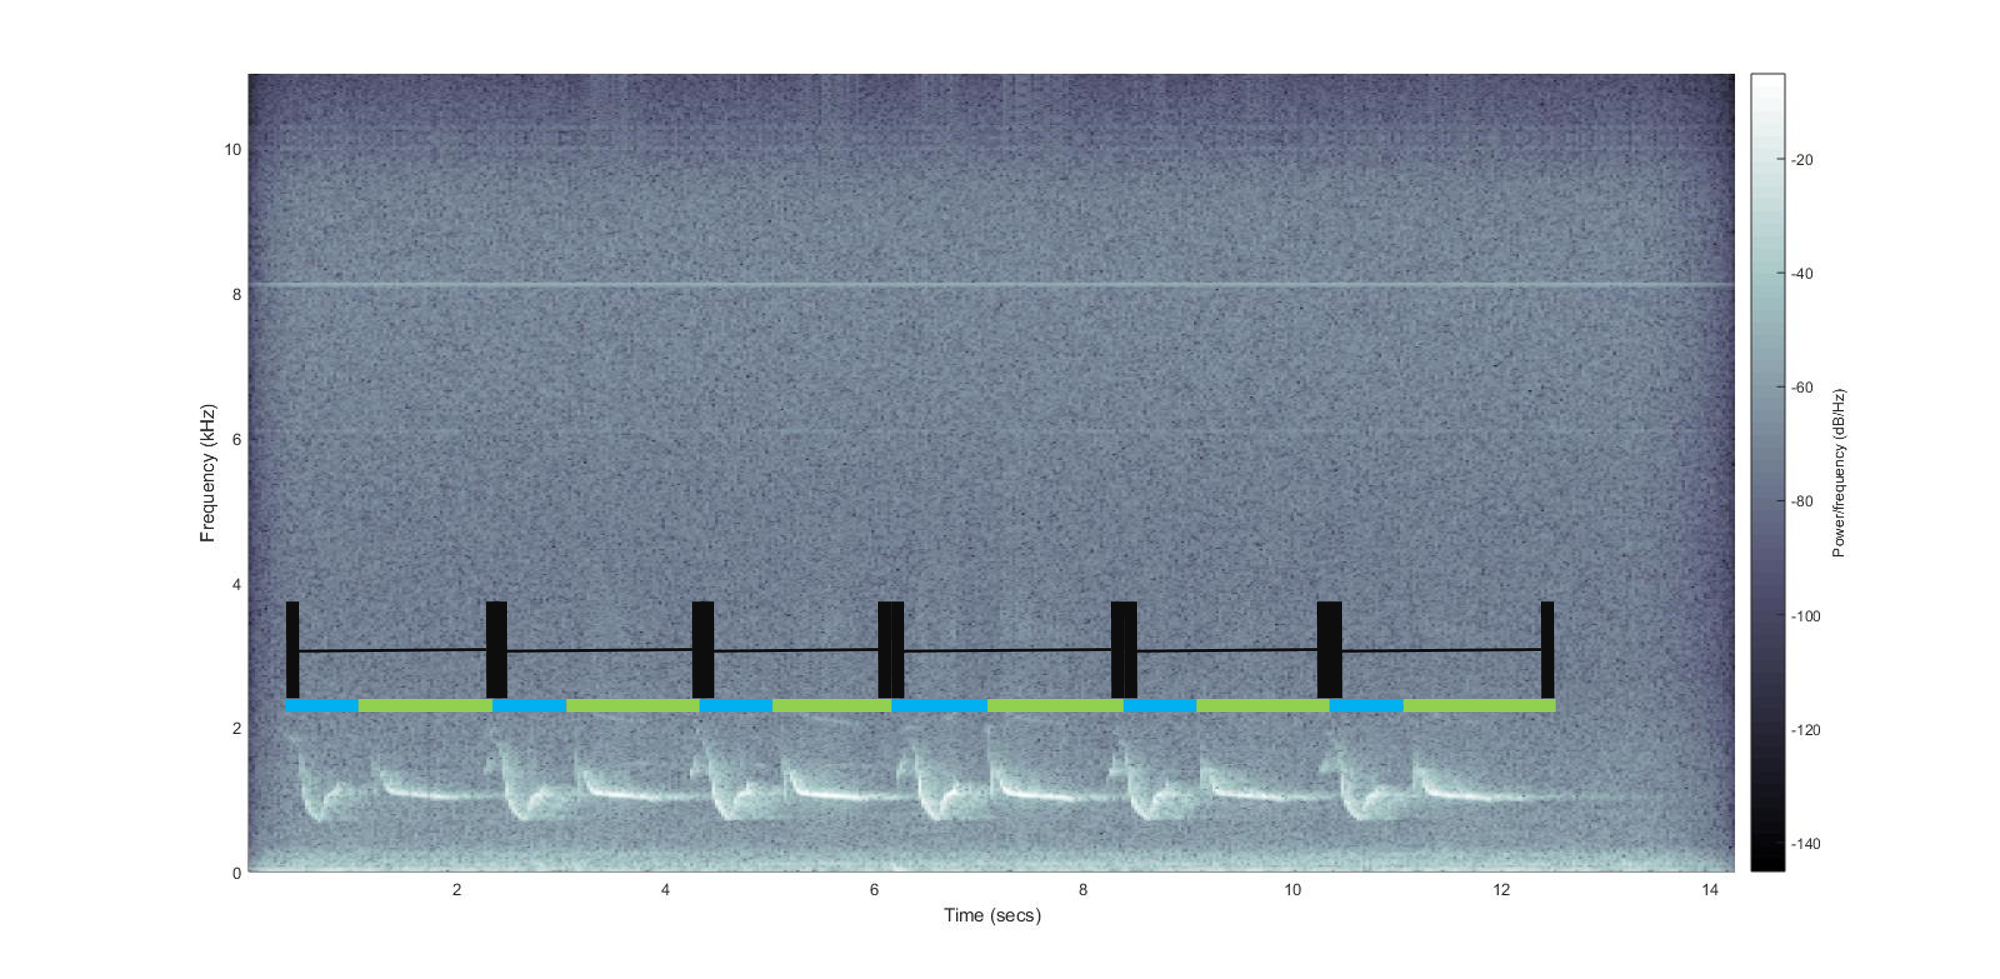
\includegraphics[width=\textwidth]{images/birdsong_structure}
\caption{Spectrogram from a birdsong recording of the species \emph{Periparus ater}. The thick blue and green bars represent syllables, and the black boxes represent a motif. Remark the pattern repeats regularly from left to right, and that motifs can be grouped hierarchically as syllables \cite{Snowdon2013}.}
\label{fig_birdsong_structure}
\end{figure}
\par Importantly, several academics in Zoology have pointed out the similarities between human speech and birdsong, e.g. we can think of both humans vowels and birdsong as ``complex, patterned vocalisations" \cite{Berwick2013,Naguib2014}. This remark enables us to analyse birdsong by means of some of the techniques from the field of Automatic Speech Recognition (ASR), which will be introduced in section \ref{section_model}. 
\par The rest of this article is organised as follows: in section \ref{section_model}, we introduce the mathematical framework used to build phylo-acoustic trees; then, in section \ref{section_results}, we present our experiments and results; and in section \ref{section_conclusion} we present our conclusions and future work.
\section{Model architecture (1500-2000 words)}
\label{section_model}

\section{Experiments and results (1500 words)}
\label{section_results}

\section{Conclusion (500 words)}
\label{section_conclusion}
\blindtext

\section*{Acknowledgments}


The authors would like to thank the National Council for Science and Technology in Mexico (CONACYT) for funding this research project.


\addcontentsline{toc}{chapter}{Bibliography}
\bibliographystyle{unsrt}
\bibliography{bib}

\end{document}


